\documentclass[conference]{IEEEtran}

\usepackage[T1]{fontenc}
\usepackage{cite}
\usepackage{amsmath,amssymb,amsfonts}
\usepackage{graphicx}
\usepackage{textcomp}
\usepackage{xcolor}
\usepackage{booktabs}
\usepackage{array}
\usepackage[hidelinks]{hyperref}
\newcommand{\todo}[2]{\par\smallskip\noindent{\color{blue!55!black}\textbf{TODO: #1.} #2}\par\smallskip}
\newcommand{\pending}{\textcolor{blue!55!black}{pending}}
\title{Agentic Goal-Conditioned Workload Synthesis for Dynamic Power Characterization}

\author{
\IEEEauthorblockN{Aman Desai}
\IEEEauthorblockA{
\textit{University of California, Santa Barbara} \\
Santa Barbara, CA, USA \\
amandesai@ucsb.edu
}
\and
\IEEEauthorblockN{Zishen Wan}
\IEEEauthorblockA{
\textit{Columbia University} \\
New York, NY, USA \\
zw3306@columbia.edu
}
}
\begin{document}
\IEEEoverridecommandlockouts
\IEEEaftertitletext{\vspace{-10pt}}
\maketitle
\begin{abstract}
Temporal power characterization requires executable workloads that produce
specified switching-activity profiles while completing required work.
Synthesizing these workloads is difficult because operation latency,
contention, and persistent state couple activity across time. We present an
agentic approach to goal-conditioned workload synthesis that combines hardware
interface descriptions with interval-level simulation feedback. A large language model (LLM)
proposes and revises complete workloads, while a fixed evaluator checks
functional correctness, work completion, deadlines, and activity tolerance in
every interval. Search uses register-transfer-level (RTL) switching activity; selected workloads undergo
separate mapped-gate power assessment. Across five designs, Gemini 3.8 Flash
satisfies the activity specification in 387 of 400 runs on time-varying targets
(96.8\%) within 128 proposals per run. Across the four non-Mesh designs, it
reduces the area under the activity-error curve by 85.9-89.8\% relative to the
best evaluated classical baseline per design. The resulting workloads provide
executable stimuli for controlled activity experiments and subsequent power analysis.
\end{abstract}

\begin{IEEEkeywords}
workload generation, dynamic power, hardware agents,
temporal activity, design automation
\end{IEEEkeywords}

\section{Introduction}
A hardware workload determines not only what a circuit computes, but also
which parts of the circuit switch and when they switch. These activity
patterns affect dynamic power, so an average alone cannot distinguish a short
burst from sustained demand or repeated changes in activity. Temporal
stressmark generation already uses controlled changes in demand to study
power-delivery behavior~\cite{kim,didt}. For a designer who wishes to examine
a particular temporal condition, power analysis is only part of the task.
The designer also needs a workload that produces that condition.

Consider a packet network that must alternate between busy and quiet
intervals while delivering its scheduled traffic. Choosing packet release
times does not fully determine when switching occurs. Contention and
backpressure can delay delivery, allowing activity from one interval to
continue into the next. Similar dependencies arise when instruction latency
shifts later processor work. The next proposal must account for both available
operations and their measured timing effects. Can an LLM use supplied interface
descriptions and interval-level errors to find better-matching workloads than
classical search within the same proposal budget?

We investigate this question across five hardware designs. An LLM proposes
complete workloads from interface descriptions and revises its proposals
using simulation feedback. Random, evolutionary, and surrogate-guided policies
use the same workload languages and proposal budgets.

During search, RTL switching activity guides workload generation without
requiring gate-level simulation for every proposal. These transition counts
serve as a search proxy, not a direct power estimate. To assess power, we replay
selected and reference workloads through the synthesized designs' interfaces.
The resulting workloads can be inspected, executed, and reused.

\begin{figure*}[t]
\centering
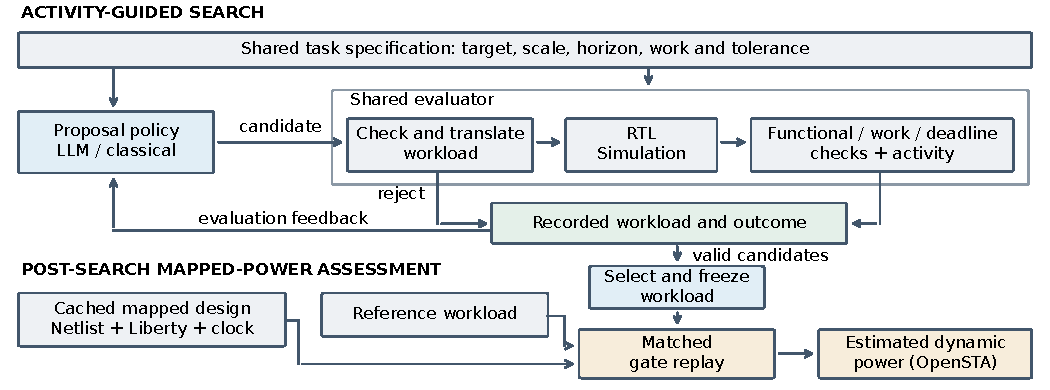
\includegraphics[width=0.95\textwidth]{figures/architecture.pdf}
\caption{Simulation feedback guides workload proposals. After search, the selected
workload and a separately constructed reference are replayed on the synthesized design under
the same conditions. Estimated power assesses the result but does not guide search.}
\label{fig:loop}
\end{figure*}

\section{Problem and Measurement}
Given a fixed design, required work, and eight interval targets, we search
for a workload that completes the work correctly and matches those targets.
We evaluate workload $w$ by simulating it on design $d$ (Figure~\ref{fig:loop}):
\begin{equation}
 \tau=\operatorname{Simulate}(d,w),\qquad
 a_k=\frac{\operatorname{Toggles}(\tau,I_k)}{C_k}.
 \label{eq:task}
\end{equation}
Here $\tau$ is the signal trace and $I_k$ contains $C_k$ clock cycles.
Toggles counts known 0-to-1 and 1-to-0 bit transitions in the measured RTL
scope, excluding clocks. Thus $a_k$ is transitions per cycle, in the same
units as the requested activity $t_k$.

\subsection{Tracking error and acceptance}
The observation period has $K=8$ consecutive intervals, or bins, with fixed
boundaries per design and lengths differing by at most one cycle. To interpret
errors on a consistent scale, we divide by a design-specific activity span
$s_d>0$: the 95th minus fifth percentile of valid calibration interval rates.
This scale stays unchanged across targets and proposals.
Signed errors describe each interval, while root-mean-square (RMS) and maximum error summarize
the profile:
\begin{equation}
 \begin{aligned}
 e_k &= (a_k-t_k)/s_d,\qquad k=1,\ldots,K,\\
 E_{\mathrm{RMS}} &= \sqrt{\frac{1}{K}\sum_{k=1}^{K}e_k^2},\qquad
 E_{\max}=\max_k|e_k|.
 \end{aligned}
 \label{eq:loss}
\end{equation}
Acceptance requires correct execution, completion of the required work on
time, and $E_{\max}\leq\epsilon=0.05$. Requiring every interval to meet the
tolerance prevents accurate matches in some intervals from compensating for
a large error in another. The tolerance is relative to the calibration span,
not a percentage of target activity or power. RMS error measures progress
toward a match.

We track the lowest RMS error among valid workloads found so far. Its
trapezoidal area under the curve (AUC) measures progress over $N=128$ proposal
slots, not elapsed time. Invalid, missing,
and duplicate proposals count toward the budget. After a successful batch,
search stops and its best error is carried forward to $N$. Unsuccessful runs
remain in the summaries. Extended methods give the full accounting convention.

\section{Goal-Conditioned Workload Synthesis}
\subsection{An executable feedback loop}
The model proposes a complete workload using the design's available operations.
An adapter checks its structure and interface constraints, then translates it
into simulator inputs. Simulation reveals when activity actually occurs.
For valid workloads, the evaluator reports which intervals have too much or
too little activity. Otherwise, it reports the rejection reason.

The next request supplies the workload format, interface description, target
and scale, and a compact history of outcomes. Errors identify what needs
improvement, while the interface description identifies possible edits.
Those edits can affect several intervals: Ibex polling waits still switch,
and earlier RedMulE jobs can delay later jobs beyond their release times.
Simulation captures these effects rather than equating workload phases with
measurement intervals. The model cannot alter the RTL or measurement rules.

\begin{table}[t]
\centering\small
\caption{Evaluated hardware interfaces and controllable workload parameters.}
\label{tab:designs}
\vspace{-2pt}
\begin{tabular}{l>{\raggedright\arraybackslash}p{0.63\columnwidth}}
\toprule
Design & Workload control \\
\midrule
OpenTitan AES & Encryption grouping and waits, fixed key/data \\
AXI DMA & Fixed-size copy grouping and pacing, no injected backpressure \\
Ibex & Instruction bodies, initial state, segment weights and releases \\
BaseJump mesh & Packet timing, routes, data patterns and sink behavior \\
RedMulE & FP16 GEMM size, operands, job counts and releases \\
\bottomrule
\end{tabular}
\vspace{-5pt}
\end{table}

\begin{table*}[t]
\centering\small
\caption{Mean AUC of best-so-far normalized RMS error and solves out of 80
nonflat runs per design. Bold marks the lowest mean AUC, not significance.
Gemini 3.8 denotes Gemini 3.8 Flash.}
\label{tab:final}
\vspace{-1pt}
\begin{tabular}{l*{5}{rr}}
\toprule
Design & \multicolumn{2}{c}{Phase-random} & \multicolumn{2}{c}{Phase-GA} & \multicolumn{2}{c}{Phase-model} & \multicolumn{2}{c}{Flash-Lite} & \multicolumn{2}{c}{Gemini 3.8} \\
 & AUC $\downarrow$ & Solves & AUC $\downarrow$ & Solves & AUC $\downarrow$ & Solves & AUC $\downarrow$ & Solves & AUC $\downarrow$ & Solves \\
\midrule
AES & 18.43 & 1 & 19.60 & 2 & 12.13 & 33 & 17.38 & 21 & \textbf{1.23} & 80 \\
DMA & 32.80 & 0 & 33.11 & 1 & 30.17 & 0 & 40.52 & 1 & \textbf{3.72} & 78 \\
Ibex & 44.86 & 0 & 41.75 & 1 & 46.91 & 0 & 51.31 & 4 & \textbf{4.86} & 80 \\
Mesh & 36.50 & 0 & 31.41 & 0 & 32.76 & 0 & 24.62 & 20 & \textbf{2.24} & 80 \\
RedMulE & 45.72 & 0 & 37.83 & 0 & 46.57 & 0 & 40.63 & 0 & \textbf{5.33} & 69 \\
\bottomrule
\end{tabular}

\vspace{-3pt}
\end{table*}

\begin{figure*}[t]
\centering
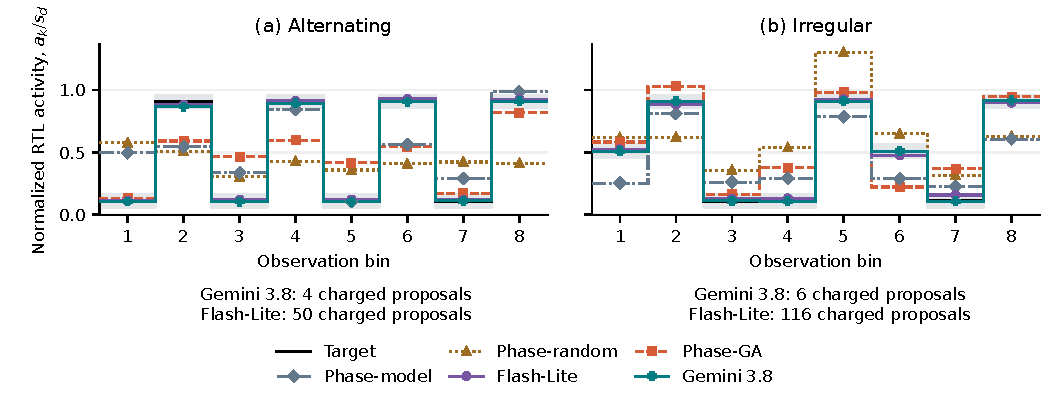
\includegraphics[width=0.9\textwidth]{figures/mesh_waveforms.pdf}
\caption{Both LLMs match these Mesh targets at seed 9100. Steps show 1,025-cycle
average activity divided by the fixed scale, not within-interval changes.
Shading marks the $\pm0.05$ tolerance. Counts include initialization and full
batches. Selection minimizes valid $E_{\max}$ with earliest-slot ties.
Classical runs use 128 slots. These are individual examples.}
\label{fig:waveforms}
\vspace{-4pt}
\end{figure*}

\subsection{Baselines with temporal control}
Mesh baselines retain sink period 8 and pauses from 0 to 3.
The LLM schema permits wider settings.
\textbf{Phase-random} samples workload phases, their timing and operations.
\textbf{Phase-GA} selects workloads using measured RMS error, then changes
their structure and timing to produce new candidates.
\textbf{Phase-model} fits ridge regression after eight valid measurements to
predict interval errors. It screens up to 32 edits using those predictions,
also includes random candidates, and favors improvements to the worst interval.
Screening uses no additional simulations, but submitted candidates consume
proposal slots. Phase-model changes selection
as well as prediction, rather than testing a predictor alone.

\subsection{Gate-level replay}
From each run, we select the valid workload with the smallest worst-interval
error, breaking ties by RMS error and earliest slot. Unsuccessful runs contribute
their best valid attempt, or no measurement if none is valid. Selection precedes
power estimation so that power cannot influence the choice.

Because an activity target does not uniquely determine power, we compare
selected workloads with separately constructed references. Both run on the same
synthesized design with the same library, 10 ns clock, and intervals. OpenSTA
estimates internal and switching power from gate activity and Liberty
characterization, excluding leakage~\cite{opensta}.

Normalized RMS power error (NRMSE) is the eight-interval RMS
candidate-minus-reference error divided by the reference's duration-weighted
mean dynamic power. Profiles are neither shifted nor independently rescaled.
Each reference provides one power realization of the activity target,
not a unique conversion of that target into watts.

Gate-level replay uses zero delay and omits routed parasitics and delay-induced
glitches. Since OpenSTA limits switching rates based on modeled signal transition
times, short bursts can exceed its limit even when the whole-run average does not.
Interval-level power estimates can therefore differ from the whole-run estimate.
For Ibex and RedMulE, we verify that clipping explains each discrepancy without
changing the reported power. Functional replay, alignment, finite power and
annotation checks remain required.

\section{Evaluation Design}
Each design has eight time-varying (nonflat) targets and a near-flat control.
Ten seeds give 80 nonflat runs per design, or 400 across 40 tasks per policy.
For each target and seed, policies share two initial workloads and 128 proposal
slots. Both candidates in each LLM response count, even if the first matches.
Observation periods span 6,774 to 262,144 cycles. Work requirements prevent
quiet matches obtained by omitting work.
Targets include steps, bursts, quiet intervals, alternation, ramps and irregular
levels. Calibration measurements set their amplitudes. AES and DMA preserve
mean requested activity across shapes, so bursts request more activity in fewer
intervals.

Gemini 3.5 Flash-Lite and Gemini 3.8 Flash use MEDIUM reasoning, temperature
0.7 and top-p 0.95, with output-token allowances of 8,192 and 65,536 respectively.

RTL simulation uses Verilator, except for DMA's Icarus flow. Yosys/Slang
synthesizes to Sky130 HD at typical 25$^\circ$C, 1.8 V. Released CHIA bindings
expose tool stages, while scores use the frozen benchmark evaluator.

For each design, we average paired AUC differences across eight targets per
seed. Ten averages support bootstrap intervals and exact sign-flip tests.
We adjust p-values across each LLM's 15 baseline comparisons to limit
the chance of any false-positive finding in that group to 5\%.
Evaluation uses an already-observed bank, not fresh held-out tasks.


\section{Results and Gate-Level Power Assessment}
\label{sec:results}
\subsection{Completed Search Comparisons}
Gemini 3.8 Flash matches 387 of 400 nonflat runs, compared with 46 for
Flash-Lite and 1, 4, and 33 for Phase-random, Phase-GA, and Phase-model
(Table~\ref{tab:final}). It also finds better activity matches earlier in
search, reducing mean error-curve AUC by 85.9\% to 92.9\% relative to the
lowest-AUC classical baseline on each design. All 15 baseline comparisons
favor Gemini 3.8 and remain significant after adjustment for multiple testing.
Flash-Lite improves on the classical policies on Mesh but has higher AUC than
all of them on DMA. Gemini 3.8 also has a larger token allowance.

Across nonflat runs, Gemini 3.8 uses 6,008 charged proposals, compared with
49,290 to 51,088 for the classical policies. Counts include initialization
and unsuccessful runs. Both LLMs match the targets in Figure~\ref{fig:waveforms},
but Gemini 3.8 reaches tolerance earlier without always having smaller final error.
The illustrated Flash-Lite workload alternates 35-packet neighbor phases and
320-packet hotspot phases. All 1,420 packets complete and every interval meets
tolerance. Its 900-cycle release phases need not align with measurement bins.

Only Gemini 3.8 solves nonflat RedMulE requests. Across all designs, controls
yield 50/50 Gemini matches and 23/50 Flash-Lite matches, separate from nonflat totals.
We replay the Mesh workloads using the baselines' sink settings,
with period 8 and pauses capped at 3. All 80 Gemini and 20 Flash-Lite nonflat
matches remain within tolerance, while one Flash-Lite control no longer matches.
Mean reference-power error changes by less than 0.001 percentage point for
either model.

\subsection{Mapped-Gate Assessment}
Without gate-power feedback during search, Gemini 3.8 also lowers mean
error against reference workloads' estimated power on every design
(Table~\ref{tab:power}). All 40 nonflat references meet the activity tolerance.
Each design's power comparison includes all 80 nonflat runs per policy.
Power agreement is a comparison with those workloads,
not a separate power-target success rate.
Of 400 nonflat Gemini profiles, 399 beat the reference's constant approximation,
its eight-bin mean. Nearly flat references can have small errors without close
temporal tracking. DMA's peak-to-trough variation is 3.0\% to 4.3\% of mean power.

\begin{table}[t]
\centering\small
\caption{Mean error against the reference workload's estimated power profile
(NRMSE, \% of reference mean). Classical selects Phase-model for AES/DMA and
Phase-GA otherwise by lowest mean error. Columns share $n$ measured pairs.}
\label{tab:power}
\vspace{-2pt}
\begin{tabular}{lrrr}
\toprule
Design & Gemini 3.8 & Classical & $n$ \\
\midrule
AES & 0.956 & 8.675 & 80 \\
DMA & 0.076 & 1.031 & 80 \\
Ibex & 14.481 & 36.848 & 80 \\
Mesh & 0.670 & 1.559 & 80 \\
RedMulE & 6.143 & 24.364 & 80 \\
\bottomrule
\end{tabular}

\vspace{-5pt}
\end{table}

\section{Related Work}
Stressmark generators seek demanding power and switching conditions~\cite{stressmark,gest}.
SAGA uses predictions to reduce measurements during genetic search~\cite{saga},
while SAT-based methods construct functional switching sequences~\cite{sat}.
Our baselines use evolutionary and surrogate search, not SAT. DiffPower provides
differentiable power analysis~\cite{diffpower}, whereas we estimate power after search.

Temporal methods move beyond high average demand. Di/dt stressmarks construct
changes in current~\cite{kim,didt}, while PaTGen combines phases and adjusts
their timing to reproduce performance behavior~\cite{patgen}. We study requested
activity profiles across different RTL workload interfaces. Related generation
loops pursue other objectives: TheHuzz and ChipFuzzer seek bugs~\cite{thehuzz,chipfuzzer},
and AgentDSE changes architecture rather than stimulus on fixed hardware~\cite{agentdse}.
CHIA provides composable infrastructure for such experiments~\cite{chia}.

\section{Discussion and Conclusion}
Gemini 3.8 Flash meets the activity specification in 387 of 400 nonflat runs
and lowers reference-power error on all five designs. These comparisons evaluate
complete policy configurations, not model choice alone. The Mesh replay tests
selected workloads but does not establish search performance under restricted
settings. Eight intervals leave finer timing unresolved. The resulting workloads
can be inspected and replayed to study temporal activity and assess estimated
dynamic power.
Code, workloads, and results are available at
\href{https://github.com/amanpdesai/agcws}{\textcolor{blue}{\underline{https://github.com/amanpdesai/agcws}}}.

\section*{Acknowledgment}
AI tools supported proofreading and editing of the manuscript.
AI-assisted programming tools were also used to develop the accompanying software.

\bibliographystyle{IEEEtran}
\bibliography{references}

\end{document}
